\documentclass[a4paper,fontset=none]{ctexart}

\usepackage{indentfirst}
\setlength{\parindent}{0em}
\usepackage{autobreak}
\allowdisplaybreaks
\usepackage{parskip}
\usepackage{geometry}
\geometry{top=3cm,bottom=3cm,left=2cm,right=2cm}
\usepackage{anyfontsize}

\usepackage{fontspec}
\setmainfont{STIX Two Text}
\usepackage{unicode-math}
\unimathsetup{mathrm=sym,mathbf=sym,mathsf=sym,bold-style=ISO}
\setmathfont{STIX Two Math}
\usepackage{physics2}
\usephysicsmodule{ab,op.legacy}
\usepackage{fixdif,derivative}
\newcommand{\um}{\upmu\mathrm{m}}
\newcommand{\ang}{\text{\r{A}}}
\AtBeginDocument{
    \let\uglyepsilon\epsilon
    \renewcommand\epsilon{\varepsilon}
}
\usepackage{tikz}
\usetikzlibrary{arrows.meta,angles,quotes}

\setCJKmainfont{Source Han Serif CN}[BoldFont=Source Han Sans CN Medium,ItalicFont=FZKai-Z03]

\title{\textbf{星际介质天文学作业}}
\author{张植竣}
\date{2024年4月12日}

\begin{document}

\maketitle

\begin{enumerate}
    \item[8.6]
    由(8.18)和(8.19)式得：
    \begin{align*}
        M(\mathrm{H\,I})
        &= \frac{16\pi m_{\mathrm{H}}}{3A_{ul} h\nu_{ul}} D_L^2 F \\
        &= 4.945 \times 10^7\,M_\odot \ab(\frac{D_L}{\mathrm{Mpc}})^2 \ab(\frac{F}{\mathrm{Jy \cdot MHz}}) \\
        &= 4.945 \times 10^7\,M_\odot \ab(\frac{D_L}{\mathrm{Mpc}})^2 \ab(\frac{F}{10^{-20} \mathrm{W \cdot m^{-2}}}) \\
        &= 4.945 \times 10^7 \times 15^2 \times 10^{-1}\,M_\odot \\
        &= 1.113 \times 10^9\,M_\odot
    \end{align*}

    \bigskip
    \item[29.1 (a)]
    如图，设$\mathrm{H\,I}$区域为一个平面平行层，总厚度为$2h$，对应于$N(\mathrm{H\,I}) = 6 \times 10^{20}\,\mathrm{cm^{-2}}$。

    \begin{center}
    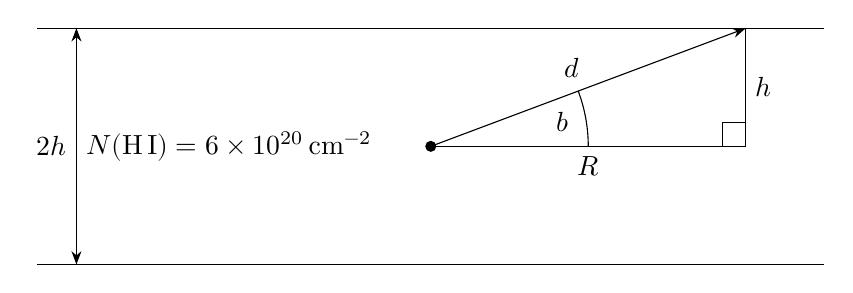
\begin{tikzpicture}[>=Stealth]
        \draw (-5,-1.5) -- (5,-1.5);
        \draw (-5,1.5) -- (5,1.5);
        \fill (0,0) circle [radius=2pt];
        \draw (0,0) coordinate (O) -- (4,0) node [midway,anchor=north] {$R$} coordinate (A) -- (4,1.5) node [midway,anchor=west] {$h$} coordinate (B);
        \draw [->] (0,0) -- (4,1.5) node [midway,anchor=south east] {$d$};
        \pic [draw,"$b$",angle radius=2cm,angle eccentricity=0.85] {angle=A--O--B};
        \pic [draw,angle radius=0.3cm] {right angle=O--A--B};
        \draw [<->] (-4.5,-1.5) -- (-4.5,1.5) node [midway,anchor=west] {$N(\mathrm{H\,I}) = 6 \times 10^{20}\,\mathrm{cm^{-2}}$} node [midway,anchor=east] {$2h$};
    \end{tikzpicture}
    \end{center}

    由于$\mathrm{H\,I}$的柱密度正比于长度，在银纬为$b$的方向，沿着视线方向的长度$d$的柱密度为：
    \[
        N(d) = N(\mathrm{H\,I}) \times \frac{d}{2h} = \frac{3 \times 10^{20}\,\mathrm{cm^{-2}}}{\sin|b|}
    \]
    由(8.11)式得：
    \begin{align*}
        \tau_\nu
        &= 2.190 \times \frac{N(d)}{10^{21}\,\mathrm{cm^{-2}}} \times \frac{100\,\mathrm{K}}{T_{\mathrm{spin}}} \times \frac{\mathrm{km \cdot s^{-1}}}{\sigma_V} \times \mathrm{e}^{-u^2/2\sigma_V^2} \\
        &= 2.190 \times \frac{0.3}{\sin|b|} \times 1 \times \frac{1}{10} \times \mathrm{e}^{-0^2/2\sigma_V^2} \\
        &= \frac{0.0657}{\sin|b|}
        < 0.5
    \end{align*}
    解得：
    \[
        |b| > 7.55^\circ
    \]

    \medskip
    \item[29.1 (b)]
    由题意，盘面半径$R$的最大值即对应$|b| = 7.55^\circ$，若$\mathrm{H\,I}$的总厚度为$2h = 300\,\mathrm{pc}$，则：
    \[
        R_{\mathrm{max}} = \frac{h}{\tan|b|} = \frac{150\,\mathrm{pc}}{\tan(7.55^\circ)} = 1132\,\mathrm{pc}
    \]

    \medskip
    \item[29.1 (c)]
    由题意：
    \begin{align*}
        \tau_\nu
        &= 2.190 \times \frac{N(\mathrm{H\,I})}{10^{21}\,\mathrm{cm^{-2}}} \times \frac{100\,\mathrm{K}}{T_{\mathrm{spin}}} \times \frac{\mathrm{km \cdot s^{-1}}}{\sigma_V} \times \mathrm{e}^{-u^2/2\sigma_V^2} \\
        &= 2.190 \times \frac{N(\mathrm{H\,I})}{10^{21}\,\mathrm{cm^{-2}}} \times 1 \times \frac{1}{10} \times \mathrm{e}^{-u^2/2\sigma_V^2} \\
        &= \frac{0.219 N(\mathrm{H\,I})}{10^{21}\,\mathrm{cm^{-2}}} \mathrm{e}^{-u^2/2\sigma_V^2}
        < 0.5
    \end{align*}
    而$\mathrm{e}^{-u^2/2\sigma_V^2}$的最大值即为谱线中心速度$u = 0$处：
    \[
        \mathrm{e}^{-u^2/2\sigma_V^2} \leqslant \mathrm{e}^{-0^2/2\sigma_V^2} = 1
    \]
    故只需要考虑：
    \[
        \frac{0.219 N(\mathrm{H\,I})}{10^{21}\,\mathrm{cm^{-2}}} < 0.5
    \]
    解得：
    \[
        N(\mathrm{H\,I}) < 2.283 \times 10^{21}\,\mathrm{cm^{-2}}
    \]

\end{enumerate}

\end{document}